Teniendo en cuenta que no existe una teoría o mecanismo formalmente establecido para la auditoría específica de compiladores, más allá de lo presentado en el capítulo anterior, podría pensarse que existen varias maneras de realizar dicha tarea.\\

Una de las maneras más sencillas de auditar el proceso, de transformar el código fuente a un ejecutable, sería generar binarios para el mismo código fuente de un lenguaje, mediante distintos compiladores, y comparar los resultados.\\

También se podría generar un mismo compilador, con distintos compiladores, para una misma arquitectura, y observar si las distintas optimizaciones aplicadas sobre el mismo compilador hacen que las generaciones realizadas por el resultante difieran tras realizarle un análisis estático.\\

Clarificación con un ejemplo. Como primer paso, se compila el código fuente para \textbf{gcc} utilizando dos compiladores distintos, \textbf{gcc} y \textbf{clang}; por lo tanto, ambos deberían devolver un ejecutable cada uno, en este caso \textbf{gcc-gcc} y \textbf{gcc-clang}. Luego, una de las maneras más sensatas de corroborar que sus lógicas son idénticas es compilar el mismo archivo con ambos compiladores resultantes, y comparar sus resultados. Como la lógica, en teoría, es la misma, ambos deberían manifestarse de la misma manera, y de hallar alguna diferencia en el programa resultante se comprobaría que alguno falló, probablemente por optimizaciones con comportamiento inesperado.\\

A continuación se presenta una selección de proyectos con las propuestas más interesantes que se encuentran en el marco de esta investigación. La mayoría de las propuestas están presentadas mediante una combinación de traducciones, adaptaciones, e interpretaciones de los artículos originalmente publicados, incluyendo un análisis de sus herramientas, en el caso de estar públicas.

\section{CSMith (2009-2013)}
\textbf{CSmith} es una herramienta de generación de casos de test randomizados, utilizada para encontrar errores en compiladores durante 5 años. A diferencia de herramientas antecesoras, \textit{Csmith} genera programas que cubren un gran subconjunto del lenguaje \textit{C}. Evita los comportamientos indefinidos y no especificados que podrían destruir la habilidad de encontrar automáticamente bugs por código erróneo. \\

Todos los compiladores que se testearon con esta herramienta se detuvieron inesperadamente (\textit{crash}), y también silenciosamente generaban código erróneo cuando eran presentados con input válido.\\

\begin{lstlisting}[language={c}, label={lst:gcc vulnerable code}, caption={Código que produjo bug en GCC}, captionpos={b}, frame={shadowbox}]]
int foo (void) {
    signed char x = 1;
    unsigned char y = 255;
    return x > y;
}
\end{lstlisting}

El código del Recuadro \ref{lst:gcc vulnerable code} pertenece a un bug hallado en una versión de \textit{GCC} incluído con \texttt{Ubuntu Linux 8.04.1} para \texttt{x86}. En todos los niveles de optimización compilaba esa función  de forma que en su ejecución retorne el valor ``1"; cuando el resultado correcto es ``0". Lo que sucedió fue que el compilador de \textit{Ubuntu} había sido fuertemente modificado a través de lo que se conoce como “parche”, ya que la versión base de \textit{GCC} no poseía ese bug\cite{Yang:2011:FUB:1993316.1993532}.\\

\textit{Csmith} genera un programa en \textit{C}; luego un código de prueba (conocido como ``arnés de prueba") compila ese programa utilizando diversos compiladores, ejecuta los ejecutables, y compara las salidas. A pesar de que esta estrategia ya había sido utilizada previamente \cite{Eide:2008:VM:1450058.1450093}\cite{McKeeman98differentialtesting}\cite{Sheridan2007c99comparison}, las técnicas de generación de \textit{Csmith}, para ese momento, avanzaron sustancialmente el estado del arte generando programas aleatorios que son expresivos—conteniendo código complejo utilizando muchas de sus características—mientras también aseguraban que cada programa generado tenga una sola interpretación. Para poder hacer esto, un programa no debe poder ejecutar ningún tipo de comportamientos indefinido, ni debe depender de ninguno de los 52 tipos de comportamiento no especificado que están descritos en el estándar C99\cite{openstdc99}.\\

Los autores de la herramienta claman que \textit{Csmith} es efectiva para buscar bugs, en parte porque genera casos de testeo que exploran combinaciones atípicas del lenguaje. Que sea código atípico no significa que no sea importante, sin embargo; no se encuentra bien representado en las suites de testeo existentes. Los desarrolladores que se aventuran fuera de los caminos más testeados que representan lo que podría denominarsela ``zona de confort" del compilador -- por ejemplo escribiendo un kernel o sistemas embebidos, utilizando opciones de compilación esotéricas (de uso extremadamente específico), o generando código automáticamente -- pueden encontrarse bugs bastante frecuente.\\

Este proyecto comenzó como un \textbf{fork} (bifurcación) de \textbf{Randprog}\cite{randprog}, un proyecto ya existente que genera programas aleatorios en \textit{C} de 1600 líneas de código. En sus trabajos tempranos extendieron y adaptaron \textit{Randprog} para encontrar bugs en la parte de la traducción de accesos a objetos calificados de volátiles, lo que dió como resultado a un programa de 7000 líneas de código. \\

Los autores convirtieron \textit{Randprog} en \textit{Csmith}, un programa \textit{C++} de 40.000 líneas para generar programas de \textit{C} aleatorios. En comparación con \textit{Randprog}, \textit{Csmith} puede generar programas de \textit{C} que utilizan una gama mucho más amplia de características de \textit{C}, incluido el flujo de control complejo y estructuras de datos como punteros, matrices y estructuras.\\

El programa \textit{Csmith} utiliza pruebas diferenciales aleatorias. Las pruebas aleatorias\cite{pinho2006reliable}, también llamadas \textit{fuzzing}\cite{Miller:1990:ESR:96267.96279}, consisten en un método de test \textit{black box} en el que las entradas de prueba se generan aleatoriamente. Las pruebas diferenciales aleatorias\cite{McKeeman98differentialtesting} tienen la ventaja de que no se necesita un \textit{oráculo} (principio heurístico o mecanismo por el cual podremos reconocer un problema, y determinar si es correcto o no). para los resultados de las pruebas. Explota la idea de que si uno tiene implementaciones deterministas múltiples de la misma especificación, todas las implementaciones deben producir el mismo resultado de la misma entrada válida. Cuando dos implementaciones producen salidas diferentes, una de ellas debe ser defectuosa. Dadas tres o más implementaciones, un evaluador puede usar el voto para determinar heurísticamente qué implementaciones son incorrectas. La Figura \ref{fig:csmith compilers} muestra cómo usaron estas ideas para encontrar errores de compilación.\\

\begin{figure}[ht]
    \centering
    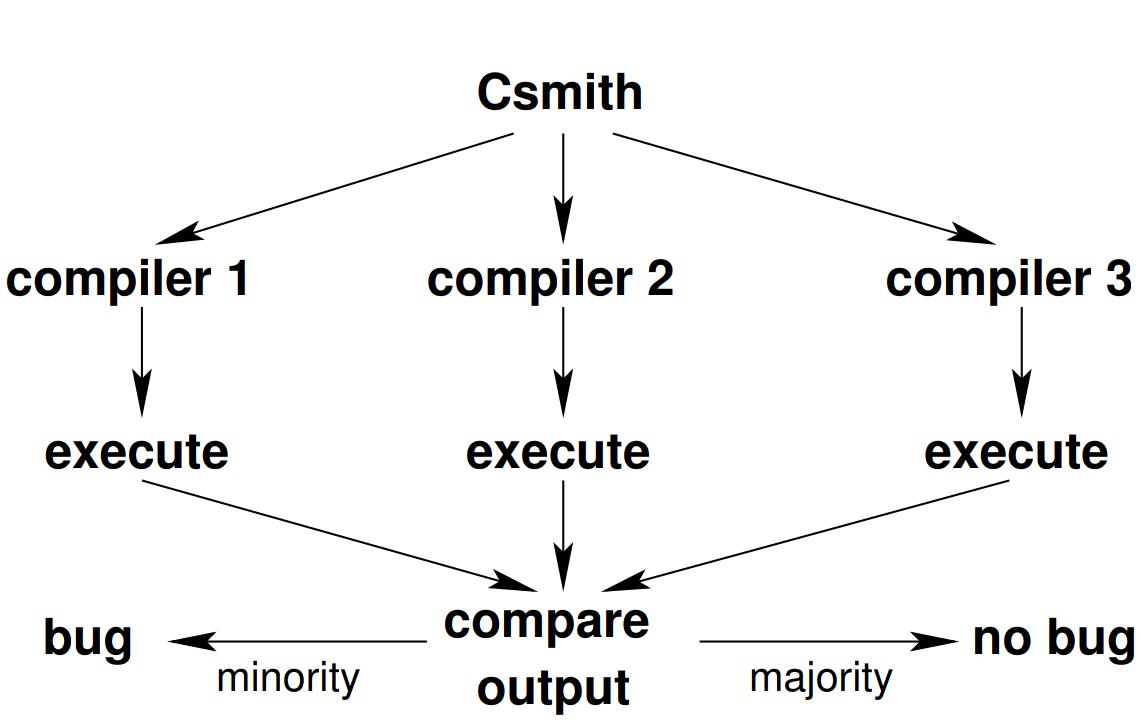
\includegraphics[scale=0.3]{images/csmith1.png}
    \caption{Ejecución en distintos compiladores}
    \label{fig:csmith compilers}
\end{figure}

\subsection{Resultados obtenidos}
Desde el año 2009 al 2013 encontraron 476 bugs en \textit{GCC}\cite{gccbuglistcsmith} y \textit{LLVM}\cite{llvmbuglistcsmith}.\\

La lista de bugs es accesible desde su repositorio\cite{bugsreportedcsmith} en \textit{GitHub}, también desde el sitio del departamento de Ciencias de la computación de UTAH.\\

El proceso de testear al azar es útil pero posee desventajas: no se puede saber cuándo dejar de testear; optimizar las probabilidades no es trivial; generar salidas expresivas que sean realmente correctas no es sencillo; y finalmente, es limitado al lenguaje. \textit{Csmith} declara ser el ataque que utiliza como técnica al \textit{fuzzing}, como el más extensivo en comparación con los compiladores de su época.\\

\textit{Resumidamente, la función de CSMith es aplicar técnicas de fuzzing el compilador utilizando programas generados al azar basados en la gramática, del lenguaje C, interpretando los resultados.}

\section{DeepSmith (2018)}
\label{ref:deepsmith}
Los autores de la herramienta presentan \textbf{DeepSmith}\cite{Cummins:2018:CFT:3213846.3213848}, como un novedoso enfoque de aprendizaje automático para acelerar la validación del compilador a través de la inferencia de modelos generativos para las entradas del compilador. Su enfoque infiere un modelo, aprendido de la estructura de código real basado en un gran códigos \textit{open source}. Luego, utiliza el modelo para generar automáticamente decenas de miles de programas realistas. Finalmente, aplican metodologías de pruebas diferenciales establecidas para exponer errores en los compiladores.\\

Se ha aplicado este enfoque al lenguaje de programación \textbf{OpenCL}, exponiendo automáticamente los errores en los compiladores de \textit{OpenCL} con poco esfuerzo de su lado. En 1.000 horas de pruebas automatizadas de compiladores comerciales y de código abierto, descubrieron errores en todos ellos.

\subsection{Comparación con CSmith}
\textit{CSmith} se desarrolló a lo largo de los años y consta de más de 41.000 líneas de código \textit{C++} escritas manualmente. Al unir estrechamente la lógica de generación con el lenguaje de programación de destino, cada característica de la gramática debe diseñarse de forma minuciosa y experta para cada nuevo idioma de destino.\\

Por ejemplo, adaptar \textit{CSmith} de \textit{C} a \textbf{OpenCL}\cite{Boujarwah1997CompilerTC} - \textit{una tarea que parecería ser simple} - les tomó nueve meses y 8.000 líneas adicionales de código. Dada la dificultad de definir una nueva gramática, generalmente solo se implementa un subconjunto del lenguaje.\\

Su metodología utiliza los avances recientes en \textit{deep learning} (conjunto de algoritmos de \textit{machine learning}) para construir automáticamente modelos probabilísticos de cómo los humanos escriben el código, en lugar de definir meticulosamente una gramática con el mismo fin. Al entrenar una red neuronal profunda en un corpus de código \textit{manualmente escrito}, es capaz de inferir tanto la sintaxis como la semántica del lenguaje de programación. El enfoque de los autores de la herramienta esencialmente enmarca la generación de programas aleatorios como un problema de modelado de lenguaje. Esto simplifica y acelera enormemente el proceso.\\

Lo más interesante de esto es que las herramientas \textit{infieren la sintaxis, la estructura y el lenguaje de programación}. Utilizan ejemplos del mundo real, no a través de una gramática definida por expertos. El tamaño promedio de los casos de prueba es dos órdenes de magnitud más pequeño que el estado del arte, sin ningún proceso de reducción costoso, y toma menos de un día para entrenar.\\

Los autores descubrieron un número similar de errores que el estado del arte, pero también encontraron errores que el trabajo anterior no pudo, cubriendo más componentes del compilador. Y en el modelado de código manualmente escrito, sus casos de prueba son más interpretables que otros enfoques.\\

\begin{figure}[ht]
    \centering
    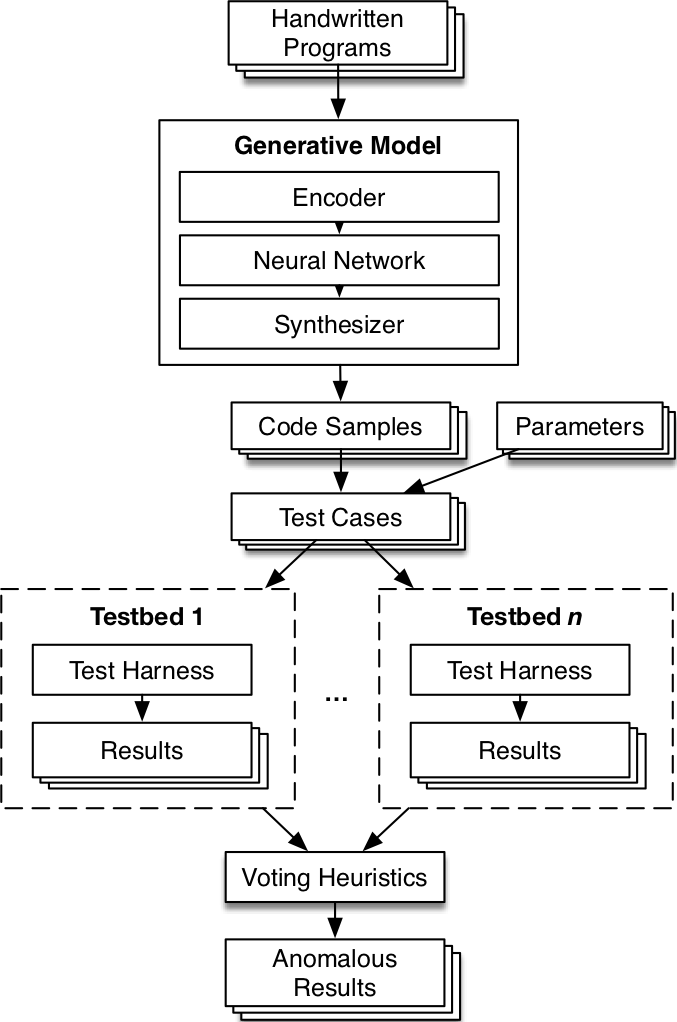
\includegraphics[scale=0.5]{images/deepsmith1.png}
    \caption{Arquitectura de DeepSmith}
    \label{fig:deepsmith architecture}
\end{figure}


\subsection{Extensibilidad del modelado de lenguajes}

Una gran parte de la arquitectura de \textit{DeepSmith} es independiente del lenguaje; ya que solo requiere un corpus, un codificador y un arnés para cada nuevo lenguaje. Esto potencialmente reduce  significativamente la barrera de entrada en comparación con los \textit{fuzzers} basados en gramática anteriores (la gran mayoría). Para explorar esto, deciden intentarlo con un lenguaje reciente, siendo este \textit{Solidity}.\\

La razón de seleccionar a \textit{Solidity}, se debe a que posee me\textit{}nos de cuatro años de desarrollo, carece de gran parte de las herramientas de lenguajes de programación más establecidos y los errores explotables pueden socavar la integridad de la \textit{blockchain} y provocar transacciones fraudulentas. 

\subsection{Resultados iniciales}
La investigación se realizó ejecutando el bucle del \textit{arnés} y el generador durante doce horas en cuatro bancos de pruebas: el ejecutable \texttt{solc} de compilación de referencia de \textit{Solidity} con optimizaciones activadas o desactivadas, y \texttt{solc-js}, que es una versión compilada por \textit{Emscripten} del compilador de \texttt{solc}.\\

Sus resultados se resumen en la tabla que muestra la Figura \ref{fig:deepsmith solc}.

\begin{figure}[ht]
    \centering
    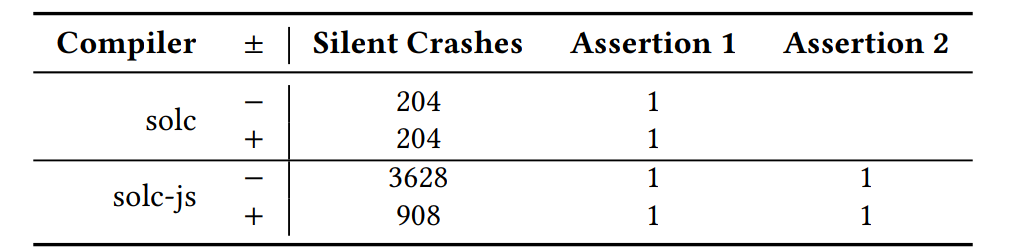
\includegraphics[scale=0.3]{images/deepsmithsolc.png}
    \caption{Resultados de testear solc y solc-js.}
    \label{fig:deepsmith solc}
\end{figure}


Los resultados de la investigación demostraron numerosos casos en los que el compilador se bloquea silenciosamente y dos aserciones distintas del compilador. El primero se debe a la falta de manejo de errores en las características del idioma (este problema es conocido por los desarrolladores). La fuente de la segunda afirmación es el tiempo de ejecución de \textit{JavaScript} y se activa solo en la versión Emscripten, lo que sugiere un error en la traducción automática de \textit{LLVM} a \textit{JavaScript}.\\

La extensión de \textit{DeepSmith} a una segunda programación requirió 150 líneas adicionales de código (18 líneas para el generador y el codificador, el resto para el arnés de prueba) y tomó aproximadamente un día. Dada la reutilización de los componentes básicos de \textit{DeepSmith}, hay un costo decreciente con la adición de cada nuevo idioma. Por ejemplo, el codificador y reescritura de \textit{OpenCL}, implementado utilizando \textit{LLVM}, podría adaptarse a \textit{C} con cambios mínimos. Dado el bajo costo de la extensibilidad, los autores de la herramienta creen que estos resultados preliminares indican la utilidad de su enfoque para simplificar la generación de casos de prueba.

\subsection{Trabajos relacionados}
La generación aleatoria de casos de prueba es un enfoque bien establecido para el problema de validación del compilador. Los enfoques anteriores se examinan en \textit{Compiler test case generation methods: a survey and assessment}\cite{Boujarwah1997CompilerTC}, \textit{Survey of Compiler Testing Methods}\cite{Kossatchev2005CompilerTM} y se contrastan empíricamente en \textit{An empirical comparison of compiler testing techniques}\cite{ComparisonCompilerTechniques}. La principal pregunta de interés es cómo generar de manera eficiente los códigos que desencadenan errores.\\

Hay dos enfoques principales: la generación de programas, donde las entradas se sintetizan desde cero; y la mutación del programa, donde los códigos existentes se modifican para identificar comportamientos anómalos.

\subsection{Programa de generación}
En el trabajo fundacional sobre pruebas diferenciales para compiladores,\textit{ McKeeman et al.} presentan generadores actuales capaces de enumerar programas de una variedad de calidades, desde secuencias \textit{ASCII} aleatorias hasta programas conformes con el modelo \textit{C}\cite{McKeeman98differentialtesting}. Los trabajos posteriores han presentado generadores cada vez más complejos que mejoran en alguna métrica de interés, generalmente expresividad o probabilidad de corrección. \textit{CSmith}\cite{Yang:2011:FUB:1993316.1993532} es un generador ampliamente conocido y efectivo que enumera programas al vincular funciones de lenguaje combinadas con poca frecuencia. Al hacerlo, produce programas correctos con un comportamiento claramente definido pero una funcionalidad muy poco probable, lo que aumenta las posibilidades de desencadenar un error.\\

Lograr esto requirió un extenso trabajo de ingeniería, la mayoría no se puede transportar a otros idiomas, e ignorar algunas características del idioma. Los generadores subsiguientes influenciados por \textit{CSmith}, como \textbf{Orange3}\cite{Nagai:Hashimoto:Ishiura}, se enfocan en características y tipos de errores más allá del alcance de \textit{CSmith}, errores aritméticos en el caso de \textit{Orange3}.\\

\textbf{Glade}\cite{Glade:Bastani:Sharma:Aiken:Liang} deriva una gramática de un corpus de programas de ejemplo. La gramática derivada se enumera para producir nuevos programas, aunque a diferencia de nuestro enfoque, no se aprende ninguna distribución sobre la gramática; la enumeración del programa es uniformemente aleatoria.

\subsection{Programa de mutación}
La prueba de entradas de módulo de equivalencia (\textit{EMI})\cite{Le:Afshari:Su:Modulo}\cite{Sun:Le:Su:Mutation} sigue un enfoque diferente para la generación de casos de prueba. Comenzando con el código existente, inserta o elimina instrucciones que no se ejecutarán, por lo que la funcionalidad debe seguir siendo la misma. Si se ve afectado, se debe a un error del compilador. Si bien es una técnica poderosa capaz de encontrar errores difíciles de detectar, se basa en tener una gran cantidad de programas para mutar. Como tal, todavía requiere un generador de código externo. De manera similar a \textit{CSmith}, \textit{EMI} favorece los programas de prueba muy largos.\\

\textbf{LangFuzz}\cite{Holler:Herzig:Zeller:Fragments} también usa la mutación, pero lo hace insertando segmentos de código que previamente han expuesto errores. Esto aumenta las posibilidades de descubrir vulnerabilidades en los motores de lenguaje de scripting.\\

La enumeración de programas esqueléticos\cite{Zhang:Sun:Su:Skeletal} funciona nuevamente al transformar el código existente. Identifica patrones algorítmicos en piezas cortas de código y enumera todas las posibles permutaciones del uso variable. Comparado con todo esto, su enfoque de \textit{fuzzing} es de bajo costo, fácil de desarrollar, portátil, capaz de detectar una amplia gama de errores y enfocado por diseño a los errores que es más probable encontrar en un escenario de producción.

\subsection{Aprendizaje automático}
Existe un creciente interés en aplicar el aprendizaje automático a las pruebas de software. Más parecido a su trabajo es \textit{Learn \& fuzz}\cite{Godefroid:Peleg:Singh:LearnAndFuzz}, en el cual una red de gran memoria de corto plazo (\textit{Long short-term memory networks}, LSTM) se entrena a través de un conjunto de archivos \textit{PDF} para generar entradas de prueba para el renderizador \textit{Microsoft Edge}, produciendo un error. A diferencia de las pruebas de compilación, los casos de prueba de \textit{PDF} no requieren entradas ni procesamiento previo del cuerpo de entrenamiento.\\

\textbf{Skyfire}\cite{Wang:Chen:Wei:Liu:Skyfire} aprende una gramática probabilística sensible al contexto sobre un corpus de programas para generar semillas de entrada para pruebas de mutación. Se muestra que las semillas generadas mejoran la cobertura del código de \textbf{AFL}\cite{AFL} cuando confunden los motores \textit{XSLT} y \textit{XML}, aunque las semillas no se usan directamente como casos de prueba. El aprendizaje automático también se ha aplicado a otras áreas, como la mejora de los analizadores estáticos de detección de errores \cite{Heo:Oh:Yi:Unsound}\cite{Koc:Saadatpanah:Jeffrey:Porter:False} la reparación de programas\cite{Koukoutos:Raghothaman:Kneuss:Kuncak}\cite{White:Tufano:Martinez:Monperrus}, la priorización de los programas de prueba\cite{Chen:Bai:Hao:Xiong:Zhang}, la identificación de \textit{buffer overruns} (sobrecargas de búfer)\cite{Choi:Jeong:Oh:Choo:BufferOverruns} y el procesamiento de informes de errores\cite{Xuan:Ming:Buggy}\cite{Lam:Anh:Nguyen:Nguyen:DeepLearning}. Según el conocimiento de los autores, ningún trabajo hasta el momento ha tenido éxito en la búsqueda de errores de compilación al explotar la sintaxis aprendida del código fuente extraído para la generación de casos de prueba. Aparentemente el trabajo de estos autores es el primero en hacerlo.

\section{Serpent by Zeppelin (Jul 2017)}

La empresa \textbf{Zeppelin}, crea herramientas para el desarrollo seguro, despliegue y operación de sistemas descentralizados. También ayudan a compañías a securizar sus sistemas \textit{blockchain} realizando auditorías.\\

La empresa \textbf{Augur} (un servicio de apuestas descentralizado) los contrató para realizarle una auditoría a \textbf{Serpent}, un compilador de un lenguaje \textit{Python-style} que compila a \textit{EVM}. El interés de \textit{Augur} en esta auditoría está dado por razones propias, tuvieron un inconveniente de seguridad por utilizar este lenguaje. El código del proyecto se puede ver aún en su repositorio de \textit{GitHub}\cite{SerpentRepository}.\\

\begin{displayquote}
    \textit{``Hemos encontrado que el proyecto Serpent es de muy baja calidad. No se ha testeado, hay muy poca documentación y el diseño del lenguaje es muy defectuoso. Serpent no debe considerarse segura de usar a menos que se solucionen muchos problemas críticos."}
    \newline{\null\hfill -- Zeppelin Research team}
\end{displayquote}

En su publicación\cite{SerpentCompilerAuditZep}, la introducción a los resultados del reporte también es utilizada como conclusión al final del mismo. El contenido de ella es una la lista con los problemas apuntando directamente al documento original que posee detalle técnico.\\

El reporte original menciona que su estrategia fue analizar el código \textit{C++} del compilador, sumado a revisar documentación, ejemplos, y herramientas recomendadas para trabajar con los contratos de \textit{Serpent}. Realizaron diversos contratos de ejemplo minimales, para verificar y exponer los problemas que encontraron. Analizaron el código assembler tanto en \textit{LLL} (Lisp Like Language, un lenguaje con un nivel de abstracción superior a la \textit{EVM}, pero considerado assembler) como en la \textit{EVM}, así como también su comportamiento en ejecución.\\

El análisis no explica metodologías ni tecnologías aplicadas a obtener a estos resultados. En base a todo lo observado el autor concluye que se trata de un proceso manual, poco automatizado, de un gran equipo. Sin embargo el acercamiento que la empresa tomó, a nivel proyecto, parece mucho más interesante que simplemente crear una herramienta, utilizar una ya existente sin explicar cómo utilizarla, o publicar los resultados sin establecer contacto con el equipo del producto analizado. Tal vez sea una diferencia destacable entre proyectos de grado y un contrato empresarial.
Fué la primera auditoría que llamó la atención del autor en su momento, y mostró tanto la importancia como el estado inmaduro del mercado en este tipo de tecnologías.\\ 

Lamentablemente la auditoría fue realizada sobre un proyecto que aparenta haber sido descontinuado mientras se publicaba ese reporte. El reporte fue presentado en Julio del 2017, y las últimas actualizaciones a Serpent fueron realizadas meses antes. Actualmente se encuentra obsoleto y sin aplicar los cambios recomendados por el equipo.


\section{Solidity by Coinspect (Nov 2017)}
Nuevamente Augur contrató otro equipo de investigadores, esta vez a Coinspect, para realizar una auditoría al compilador de Solidity.\\

Coinspect, es un equipo reconocido por sus trabajos específicamente en el ambiente de la cyber seguridad. Entendiendo esto, no es extraño encontrar en la introducción de la publicación\cite{SolidityCompilerAuditReport} un poco más de detalle\cite{SummaryCoinspectReport} sobre lo que esperan encontrar o qué piensan en buscar relacionado en términos de seguridad.\\

El equipo de Coinspect analizó la herramienta Solidity con la posibilidad de encontrar fallas del siguiente estilo:
\begin{itemize}
    \item Reducción de la seguridad de los contratos desplegados.
    \item Resultado en comportamiento no determinista.
    \item La ejecución de código malintencionado o que se bloquee al analizar el código fuente de un contrato en Solidity especialmente diseñado.
    \item Agotamiento de recursos durante la compilación, ya sea CPU, memoria o disco.
    \item Código compilado que consume una cantidad no constante de gas (por ejemplo, según los argumentos), donde el programador habría esperado un costo constante.
    \item Facilitando código malicioso (troyanos en código abierto).\newline
\end{itemize}

También buscaron vulnerabilidades comunes a vectores en aplicaciones de software:
\begin{itemize}
    \item Validación de entrada.
    \item Prevención de denegación de servicio (DoS).
    \item Prevención de la fuerza bruta.
    \item Divulgación de información.
    \item Vulnerabilidades de corrupción de memoria: buffer overflows, format strings por el usuario.
    \item Integer overflows/underflows.
    \item Vulnerabilidades de gestión de punteros: double free, user after free.
\end{itemize}


En cuanto a los resultados, exceptuando uno sólo de los problemas reportados que parece haber sido hallado mediante un proceso manual, el autor se atrevería a decir que el resto pertenecen a una clásica familia resultante de aplicar técnicas de fuzzing.\\

La diferencia principal que se podría hacer, sobre los análisis de Serpent y Solidity, es que Coinspect se enfoca principalmente en el hallazgo de vulnerabilidades y Zeppelin a problemas de diseño e implementación, los cuales a su vez pueden tener implicancias de seguridad.\\

Hay que tener en cuenta que que se hace imposible comparar con objetividad los procesos de cada equipo, dado que están meramente basadas en los resultados de cada investigación, y no se están teniendo en cuenta las herramientas disponibles, ni los recursos económicos o el tiempo que poseyó cada equipo al momento de realizarlas.\\

\section{Solidity by Ethereum Foundation}

Para situarse en contexto, el compilador de Solidity junto con su lenguaje fueron impulsados por la Ethereum Foundation. Su código está disponible en GitHub\cite{SolidityGitHub} desde sus comienzos, donde realizan releases periódicamente, tienen su documentación en ReadTheDocs\cite{ReadTheDocsSolidity}, y una amplia comunidad que colabora con el proyecto.\\

Si bien al momento de esta investigación no parecen aplicar seguridad a su SDLC, en su repositorio dicen realizar testing y fuzzing antes de cada release. Adicionalmente en su documentación se poseen categorías útiles con la intención de reducir las fallas en el código. Algunos ejemplos son patrones de diseño, código de estilo, consideraciones de seguridad, reproducción de testing, y una explicación de cómo utilizar el fuzzer que está incluido en el proyecto.\\

Varios de los bugs reportados por el equipo de Coinspect siguen sin estar corregidos, y no es posible distinguir en el sistema de reportes de tickets de github, qué bugs corresponden a su suite de testing, y de qué manera se han encontrado. Tal vez muchos errores no llegan a ser publicados mediante commits porque son testeados localmente, y esa información no se encuentra visible al público. El sitio solfuzz.ethdevops.io\cite{SolfuzzSite} solía dar estadísticas de los resultados encontrados por el fuzzer incorporado pero en el momento de este análisis se comprobó que ha dejado de funcionar hace tiempo.\\

Podrá no ser una solución similar a las demás, ya que no se dedican específicamente a aplicar seguridad o auditar el proyecto. Pero todas las soluciones apuntan a lo mismo, securizar los smart contracts através del compilador. Ésta es una tarea que principalmente el equipo de Solidity debería liderar ya que es su responsabilidad tomar los recaudos necesarios a través de su ciclo de desarrollo para proveer un servicio seguro.

\section{Discusión sobre las soluciones presentadas}
Mientras más eficiente sea la herramienta para analizar un compilador, más acoplada a su gramática deberá ser, y como consecuencia serán menos abarcativas. La adaptación de estas herramientas para poder migrar entre lenguajes es sumamente costosa.\\

En el caso de DeepSmith, los autores de la herramienta lograron aplicar su funcionalidad partiendo desde OpenCL hasta Solidity sin demasiado esfuerzo. Sin embargo, los testeos sobre los compiladores de Solidity fueron de los más breves y menos explorados que realizaron. No se buscaron impactos reales ni se hizo un chequeo sustancial sobre los hallazgos.\\

La problemática que se trata de presentar no es que el fuzzing no funciona, sino que no forman parte directa de realizar una auditoría. Se presentan como herramientas, analizan los proyectos, en este caso compiladores, y dan por finalizada la investigación. Su propósito no es encontrar y analizar las vulnerabilidades, sino proveer una herramienta para hacerlo.\\

Las dos propuestas que poseen un valor destacable, son las realizadas por las dos empresas previamente mencionadas, Coinspect y Zeppelin. Aún así son un paso accesorio a las herramientas presentadas, sólo que la herramienta en cuestión es un equipo en vez de un sólo software.\\

\textit{Las sugerencias incorporadas al reporte de Serpent por parte del equipo de Zeppelin fueron de gran motivación para realizar este proyecto.}\\

Al momento de la redacción de este documento, no se encuentra disponible una herramienta para analizar el código de compilador y entender cómo podría influir al lenguaje que ésta interpreta. En el caso de Solidity tampoco hay una gramática oficial definida de manera reutilizable, ya que el scanner no está basado en una gramática estándar, sino que está diseñada su lógica dentro del mismo parser.
Teniendo en cuenta lo descrito en el capítulo anterior, se puede concluir que las alternativas provistas e históricas en el estado del arte no son soluciones suficientes o aplicables para concluir un análisis completo, o mejor dicho una auditoría completa, al proyecto en cuestión, Solidity.
